\section{Introduction}
Radio/(sub)-millimeter (mm) telescopes are powerful tools to study the Universe at radio, sub-millimeter, and millimeter wavelengths.
These telescopes are designed to capture and detect electromagnetic radiation from space, which can provide valuable insights into astronomical phenomena,
ranging from the formation of stars \cite{Haarsma2000} and galaxies \cite{Breugel1999} to the behavior of black holes \cite{Coriat2011}.
One of the key components of a radio telescope is its reflective surface, which collects and focuses the incoming radiation.
Most radio/(sub)-mm telescopes have a large, parabolic dish-shaped primary mirror, reflecting incoming radiation onto a smaller, secondary mirror (see Figure \ref{subfig:radio_telescope}).
The secondary mirror (or subreflector) then reflects the radiation onto a detector or receiver placed at the focal point, which records and processes the signals.
In astronomy, the term "pointing" refers to the process of positioning the telescope to observe an astronomical source.
The goal is to fit the source at the center of the central resolution element or "beam" of the telescope (see Figure \ref{subfig:beamwidth}),
which in the case of single-beam instruments corresponds to the field of view of the telescope.\\

\begin{figure}[H]
    \centering
    \begin{subfigure}[t]{0.49\textwidth}
        \centering
        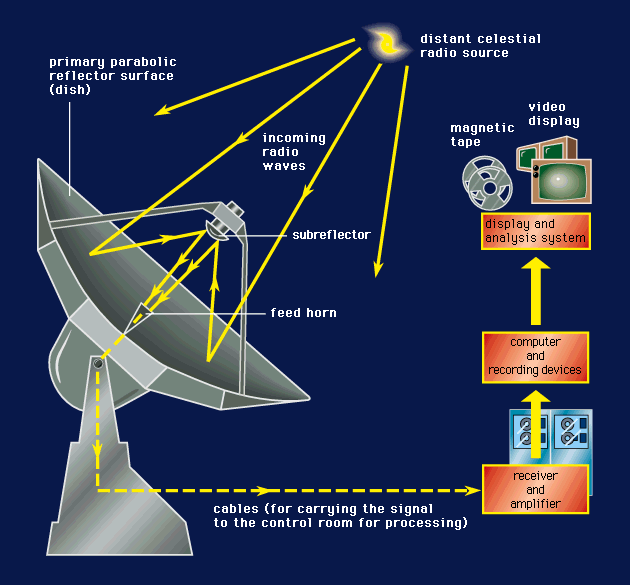
\includegraphics[width=\textwidth]{Astronomy/radio_telescope.png}
        \caption{Radio telescope basics. Source \cite{MarksPhysicsHelp}}
        \label{subfig:radio_telescope}
    \end{subfigure}
    \hfill
    \begin{subfigure}[t]{0.49\textwidth}
       \centering
       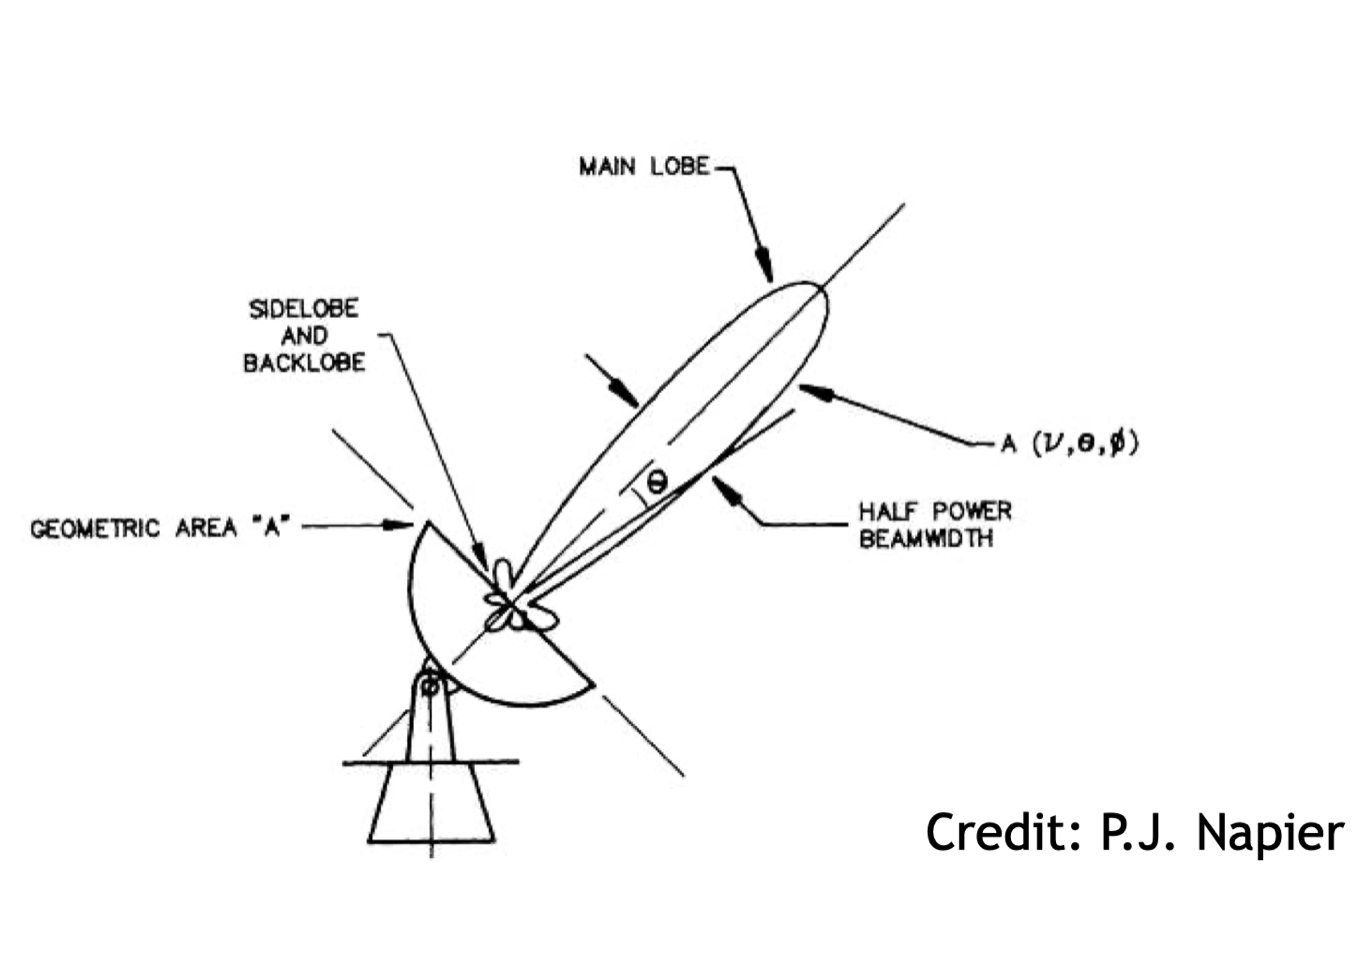
\includegraphics[width=\textwidth]{Astronomy/beamwidth_sketch_cropped.png}
       \caption{Telescope beam sketch. Source: P. Napier, Synthesis Summer School 2002 (\href{https://slideplayer.com/slide/7448846/}{https://slideplayer.com/slide/7448846/})}
       \label{subfig:beamwidth}
    \end{subfigure}
    \caption[Radio telescope basics]{\textbf{a)} Basics of how a radio telescope works and \textbf{b)} Sktech of a telescope's beam.}
    \label{fig:telescope_info}
\end{figure}


Radio/(sub)-mm telescopes detect and record photons over time, which are then processed to create a composite image or spectrum.
However, this process requires highly accurate pointing, as even slight errors in the telescope's orientation can significantly affect the resulting data quality.
Pointing errors, often referred to as pointing offsets, can be caused by various factors, including thermal deformation of the telescope components \cite{Dong2018},
gravitational deformation \cite{GravDeformation}, and other environmental factors like humidity \cite{Corstanje2017} and wind \cite{Gawronski2005}.
Most radio/(sub)-mm instruments do not have an imaging camera.
Hence, the correct positioning of the source within the resolution element (beam) and at the center of the field of view cannot be checked directly.
To achieve this accuracy, radio/(sub)-mm telescopes use pointing models \cite{stumpff1972}, which take into account a range of factors that can contribute to the pointing error,
including weather conditions, telescope structure, and the target's position in the sky.\\

The Atacama Pathfinder EXperiment (APEX) telescope \cite{APEX2006}\footnote[1]{Link to APEX website \href{http://www.apex-telescope.org/ns/}{http://www.apex-telescope.org/ns/}}, pictured in Figure \ref{fig:apex_images}, located in the high-altitude Atacama Desert in Chile,
currently uses an effective analytical pointing model run in the background and recalibrated periodically through pointing measurement campaigns.
However, there is still a residual pointing offset (with a median value of $2.84$ arcseconds and an interquartile range of $1.55$ to $4.66$ arcseconds at $230$GHz) whose origin is not understood.
This thesis aims to investigate two research questions.
First, we want to explore using machine learning to increase the pointing accuracy of the current pointing model at APEX based on observational data such as weather patterns and telescope pointing.
Secondly, we want to investigate a machine learning approach for developing a pointing model from scratch for a new radio/(sub)-mm single dish telescope.
A machine learning approach would benefit larger radio/(sub)-mm telescopes like the future Atacama Large Aperture Submillimeter Telescope (AtLAST)
\footnote[2]{Link to AtLAST website \href{https://www.atlast.uio.no/}{https://www.atlast.uio.no/}}.
AtLAST will have a $50$-meter diameter primary mirror and $12$-meter diameter subreflector. Hence, the subreflector will be as big as APEX's primary mirror.
Due to the size and complexity of AtLAST, it will be harder to develop an analytical model.
By developing a more advanced and reliable pointing model with machine learning,
this research can enhance the capabilities of current and future radio/(sub)-mm telescopes to advance our understanding of the universe.


\begin{figure}[H]
    \centering
    \begin{subfigure}[t]{0.49\textwidth}
        \centering
        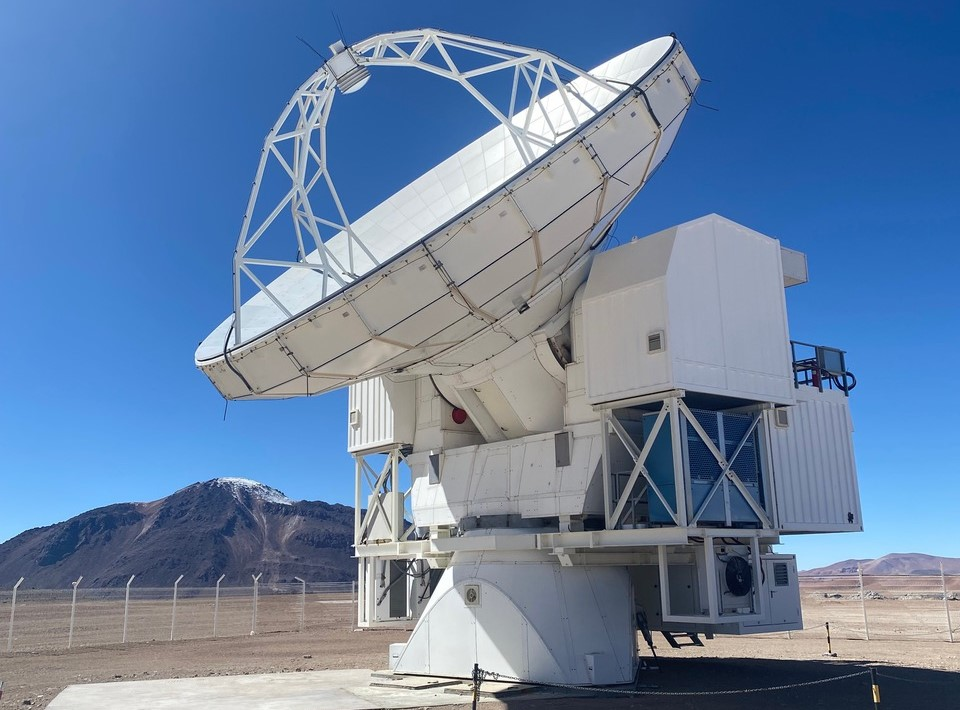
\includegraphics[width=\textwidth]{Astronomy/apex_primary_mirror_cropped.jpeg}
        \caption{Telescope structure. Credit: C. Cicone (2023)}
        \label{subfig:apex_primary}
    \end{subfigure}
    \hfill
    \begin{subfigure}[t]{0.49\textwidth}
       \centering
       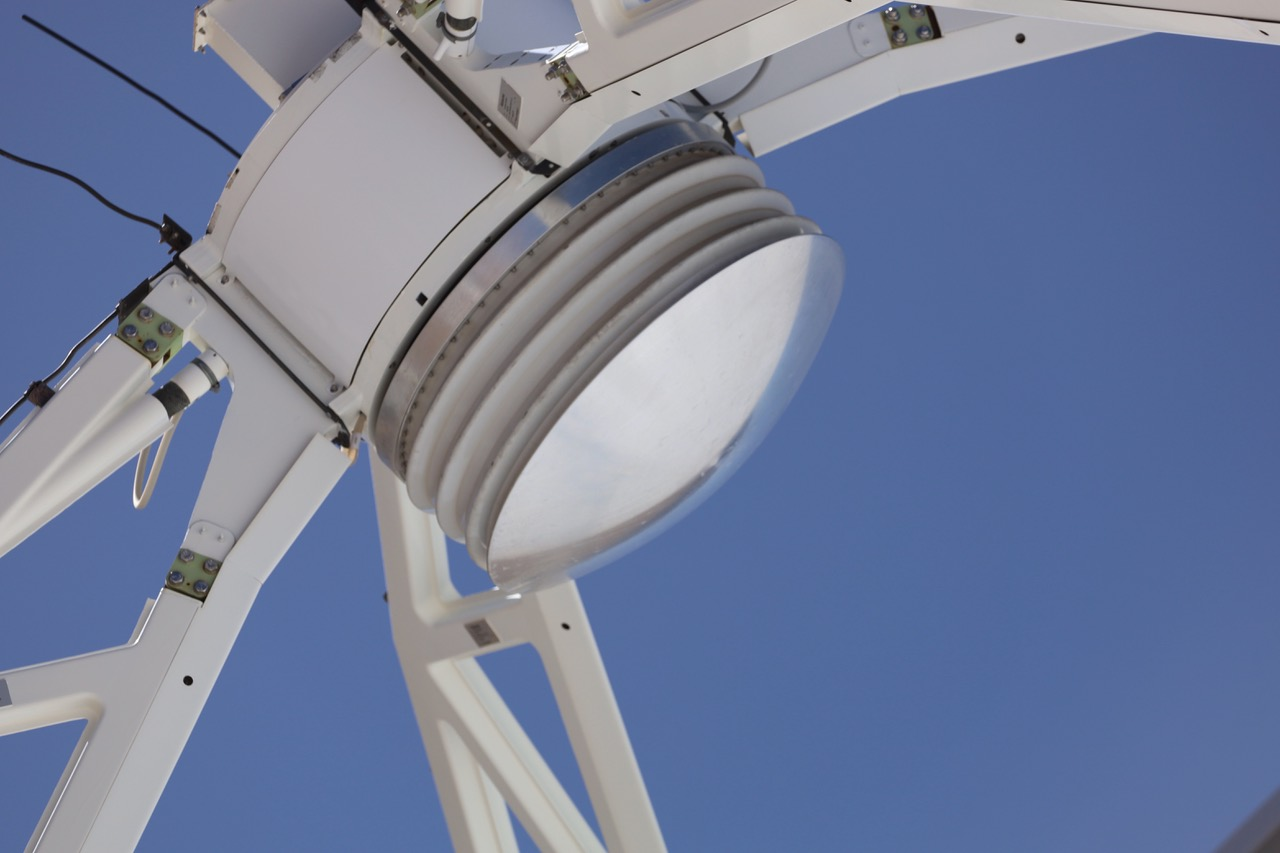
\includegraphics[width=\textwidth]{Astronomy/apex_subreflector.jpeg}
       \caption{Subreflector. Credit: P. Gallardo (2023)}
       \label{subfig:apex_subref}
    \end{subfigure}
    \caption{Pictures of the APEX telescope}
    \label{fig:apex_images}
\end{figure}
